\pagestyle{empty}
\thispagestyle{empty}
\chapter{Методы второго порядка}

\textbf{Задача коммивояжера} является классической задачей комбинаторной оптимизации. Необходимо найти самый короткий маршрут, проходящий через $n$ городов ровно один раз и возвращающийся в исходный город. Формально задача формулируется следующим образом:

\begin{equation}
    \min_{\pi \in S_n} \sum_{i=1}^{n} c_{\pi(i)\pi(i+1)},
    \label{eq:tsp}
\end{equation}

где $S_n$ --- множество всех перестановок $n$ городов, $\pi(i)$ --- $i$-й город в перестановке, $c_{ij}$ --- стоимость перемещения из города $i$ в город $j$.

\begin{figure}[h!]
    \centering
    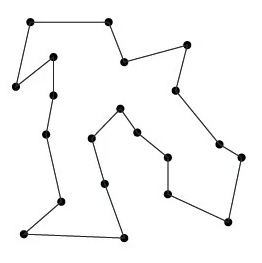
\includegraphics[scale=0.6]{img/zadanie_cas/1-route.png}
    \caption{Пример маршрута коммивояжера}
    \label{fig:tsp_example}
\end{figure}

\section{Метод Ньютона}

Метод Ньютона использует матрицу Гессе для нахождения точки минимума функции. На каждом шаге итерации решается система линейных уравнений, которая определяет направление и длину шага.

\section{Метод BFGS}

Метод BFGS (Broyden-Fletcher-Goldfarb-Shanno) является квазиньютоновским методом, который основан на последовательных непрерывных приближениях задачи с использованием аппроксимации матрицы Гессе.

\section{Основные свойства методов второго порядка}

\textit{Квадратичная сходимость} --- методы второго порядка быстро приближаются к оптимальному решению в окрестности экстремума, обеспечивая квадратичную скорость сходимости.

\textit{Точность} --- с помощью вторых производных метод учитывает кривизну функции и более точно определяет направление поиска.

\textit{Вычислительная сложность} --- вычисление и хранение матрицы Гессе требует значительных вычислительных ресурсов.